% Load document class

% possible options: color/nocolor, english/german, threecolumn
% default: color, english
\documentclass[english, leagacyboxes, nologo]{latex4ei/latex4ei_sheet}

\begin{document}
\title{Network Security}
\author{Stephan Dollberg, Martin Zellner, Lucas Vandroux}
\myemail{lucas.vandroux@gmail.com}      % optional, delete if unchanged
\mywebsite{www.latex4ei.de}     % optional, delete if unchanged
\maketitle
\section{Introduction}

  \sectionbox{
  \subsection{Security Trends}
    Network security is an issue since \emph{critical infrastructures} in the open systems with a growing user base (\ra \emph{increasing risk}) are threatend by \emph{organized crime}.
  }
  \sectionbox{
  \subsection{Security Threats}
    \textbf{Asymmetric Threat:} Defenders must protect against all exploits on all systems but attackers can attack only a few.

    \textbf{Attacker Motivation:} Ego, Revenge, Destruction, Criminal intend, Aquisition of resources, Acquistion of sensitive information
  }
  \sectionbox{
  \subsection{Security Concepts}
    \textbf{CIA Triad}
    \begin{itemize}
      \item Confidentiality (prevention of unauthorized disclosure)
      \item Integrity (prevention of unauthorized modification or deletion)
      \item Availability (prevention of unauthorized withholding)
     \end{itemize}

     Also: Authenticity, Accountability(Responsability), Nonrepudiation (Can't deny), Privacy

     (Classification by Steve Kent)
     \textbf{Passive attacks:} Confidentiality (Content compromise, Traffic analysis)

     \textbf{Active attacks:} Availabilty (Denial of service), Integrity and Authenticity (Modification, Replay, Fabrication)

     \textbf{Secure Channel:} secure = authentic (of the sender) and confidential (no eavesdropping)

     \textbf{Security on OSI-Layers:} Physical (Link encryption), Network (IPSEC), Transport (SSL), Application (SSH)
   }


\section{(In)securtity, Risk and the Lifecycle of Vulnerablities}

  \sectionbox{
  \subsection{(In)security Landscape}
    General: complexity is bad (but increases fast)

    Security of a system := Security of its weakest link
  }
  \sectionbox{
  \subsection{Vulnerablity Lifecycle}
    \textbf{Security vulnerability} \\
    a weakness in a system allowing an attacker to violate the confidentiality, integrity, availability of the system or the data and applications it hosts

    disagreement on what is a vulnerability possible (it's a a feature not a vulnerability)

    \textbf{CVE}
    Standard names for all publicly known vulnerabilities and security exposures. De facto standard.

    Form: \emph{CVE-Year-AnyDigits}

    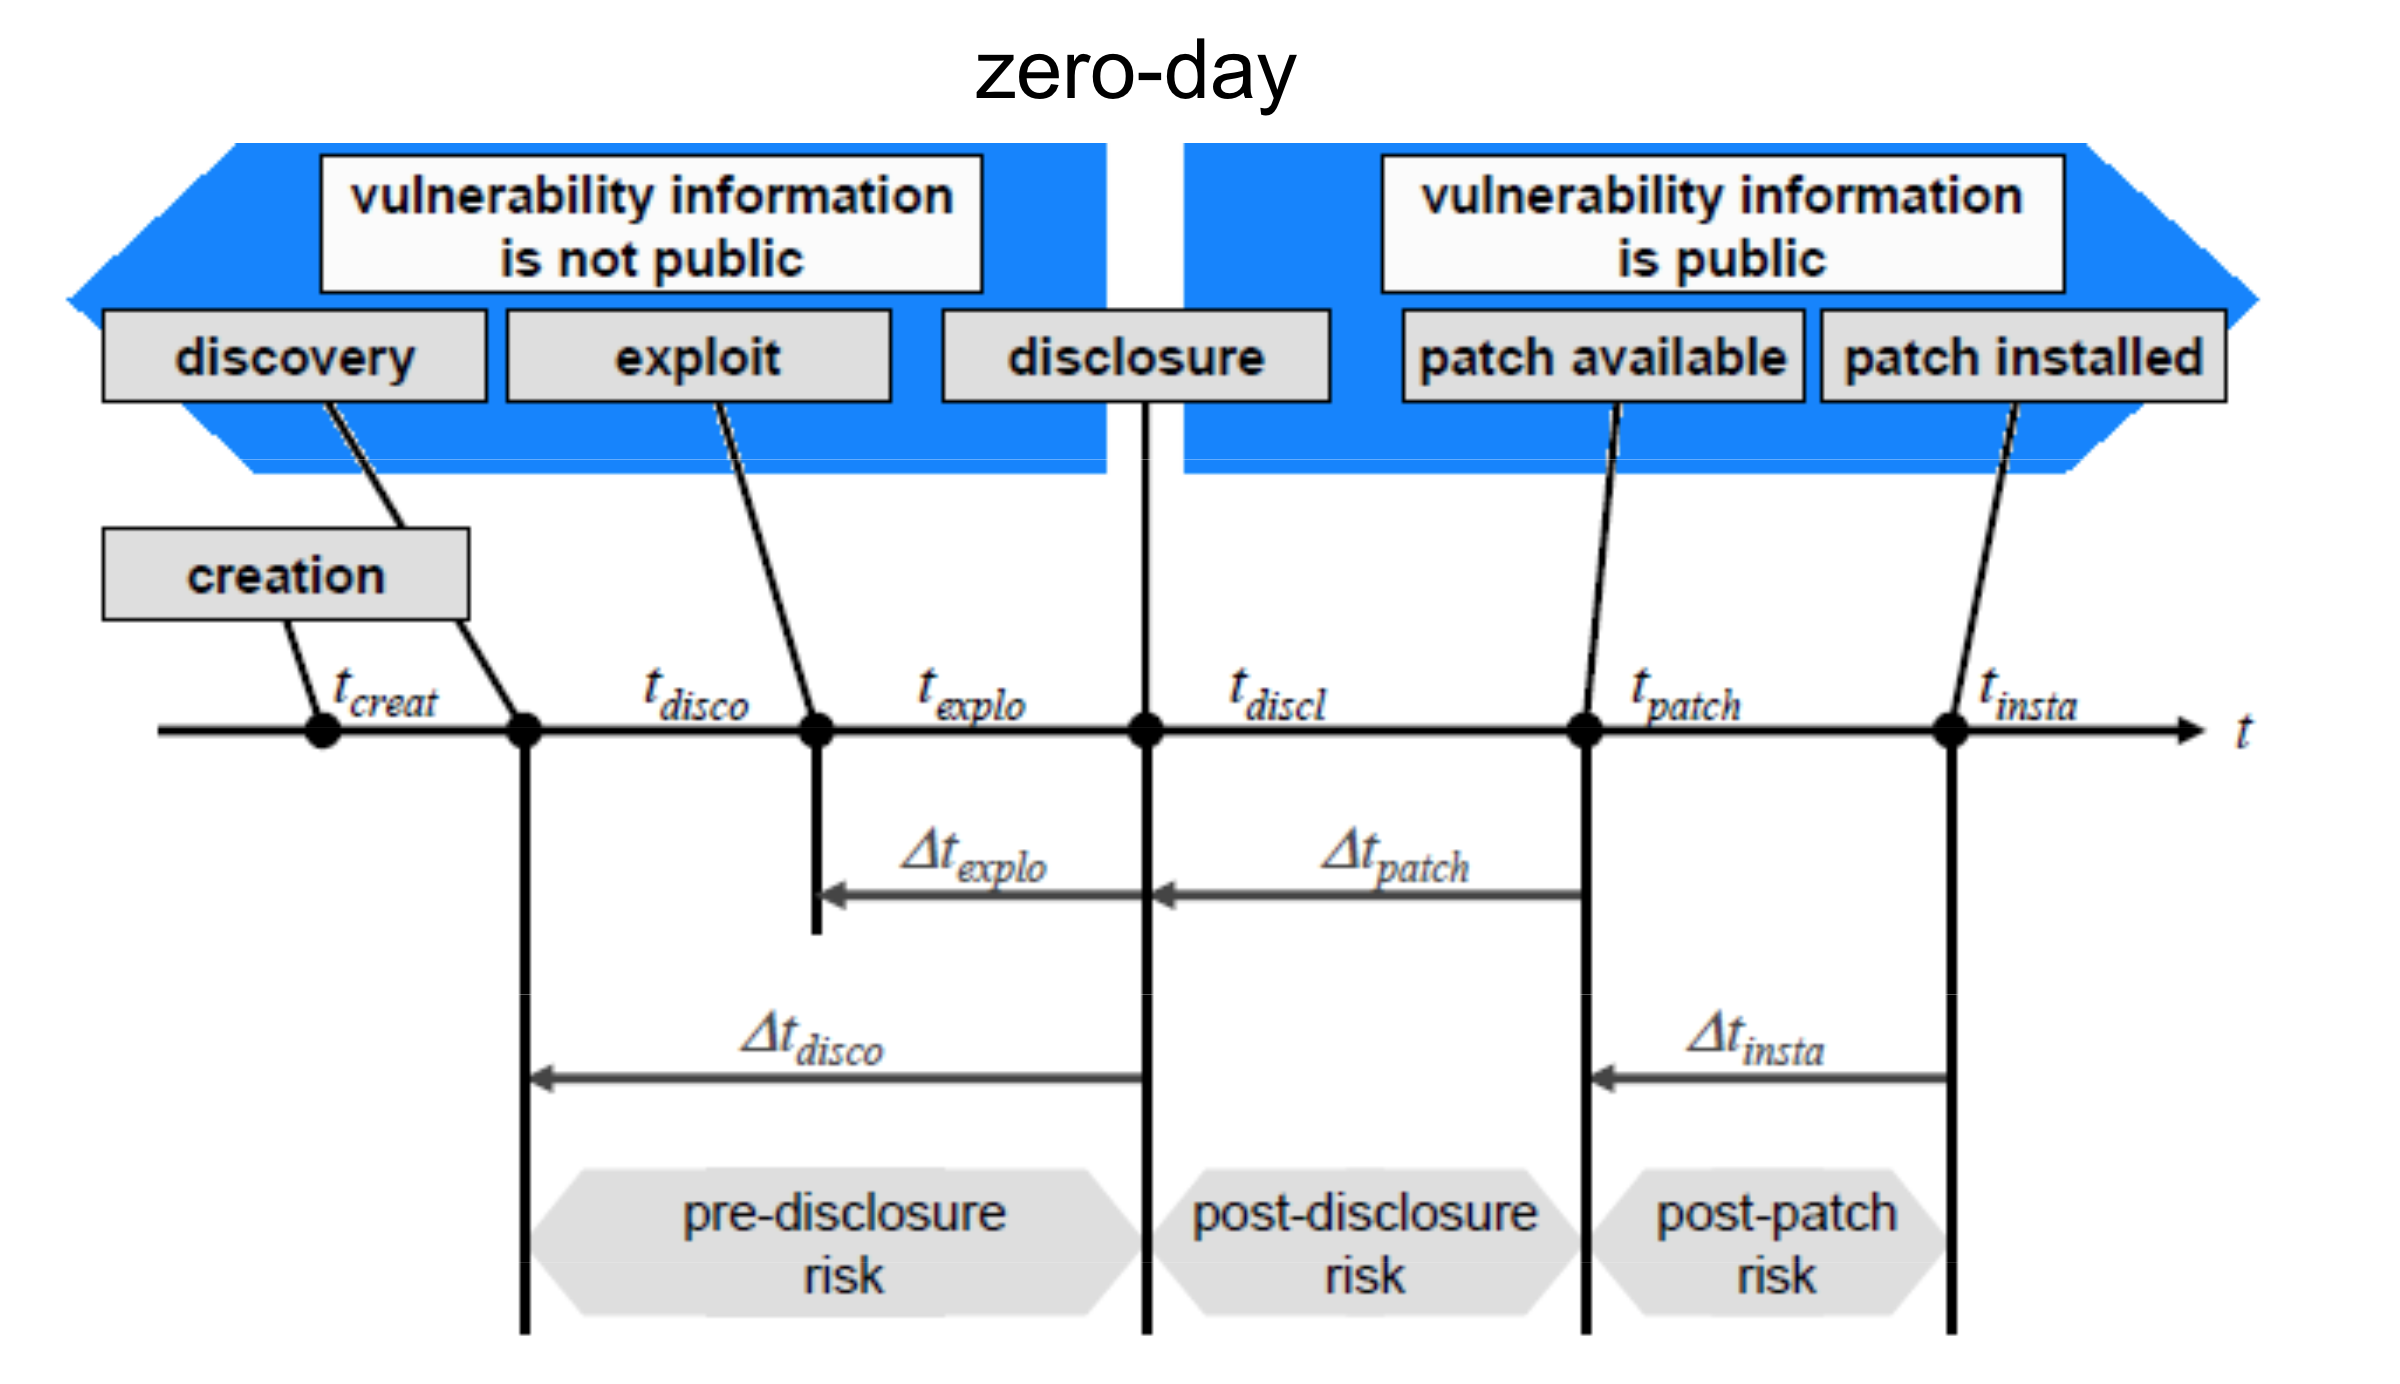
\includegraphics[width=\columnwidth]{img/VUL-LC.png}

    \textbf{Numbers:}\\
    50 \% of vulnerabilities known to insiders 30 or more days before disclosure (less-than-zero-day)

    At disclosure:  $\approx 50 \%$ unpatched

    A month after disclosure: $\approx 50 \%$ unpatched \\

    \textbf{Zero-day} Date when the vulnerability becomes known by the public

    \textbf{Zero-day-exploit} Attack that exploits a previously unknown vulnerability
  }
  \sectionbox{
  \subsection{Dynamics of (In) Security}
    \begin{itemize}
      \item extremely high dynamics around the disclosure
      \item exploit availability stays higher than the patch availability
      \item insiders: may know undisclosed vulnerabilites
    \end{itemize}

    \textbf{Gap of insecurity:} Difference between the exploit and patch (the bad a consistently faster than the good)
  }

  \sectionbox{
  \subsection{Risk}
    There is such thing as absolute security

    Trade-Off between security and financial, social, functional, \ldots

    \subsubsection{Risk analysis}
    \begin{itemize}
      \item What assets are we trying to protect?
      \item what are the risk to those assets?
      \item How well does the security solution mitigate those risks?
      \item What other risks does the security solution cause?
      \item What costs and trade-offs does the security solution impose?
    \end{itemize}
    \ra is the trade-off worth if?

    \subsubsection{Risk management}
    Security is relative \Ra manage risks

    Options: avoid, decrease, transfer, accept risk

    Business sense: risk $<$ opportunity
  }


\section{Identity and Authentication}
  \sectionbox{
  \subsection{Identity and Identity Theft}
    \textbf{Authentication:} Authentication is the process of verifying an identity claim of an entity. It binds the principal to an identity

    \textbf{Criteria:}
    \begin{itemize}
      \item Something an entity knows (e.g. password, PIN)
      \item Something an entity has (e.g. key, card)
      \item Something an entity is (e.g. biometric characteristic)
      \item rarely used: location, ability
    \end{itemize}

    \textbf{Weak authentication:} checking only one authentication criteria

    \textbf{Strong authentication:} checking two or more authentication criteria
  }
  \subsection{Authentication Protocols}
  \sectionbox{
  \subsubsection{OpenID}
    Standard for decentralised user authentication:
    use existing account to sign in to multiple websites without creating a new password

    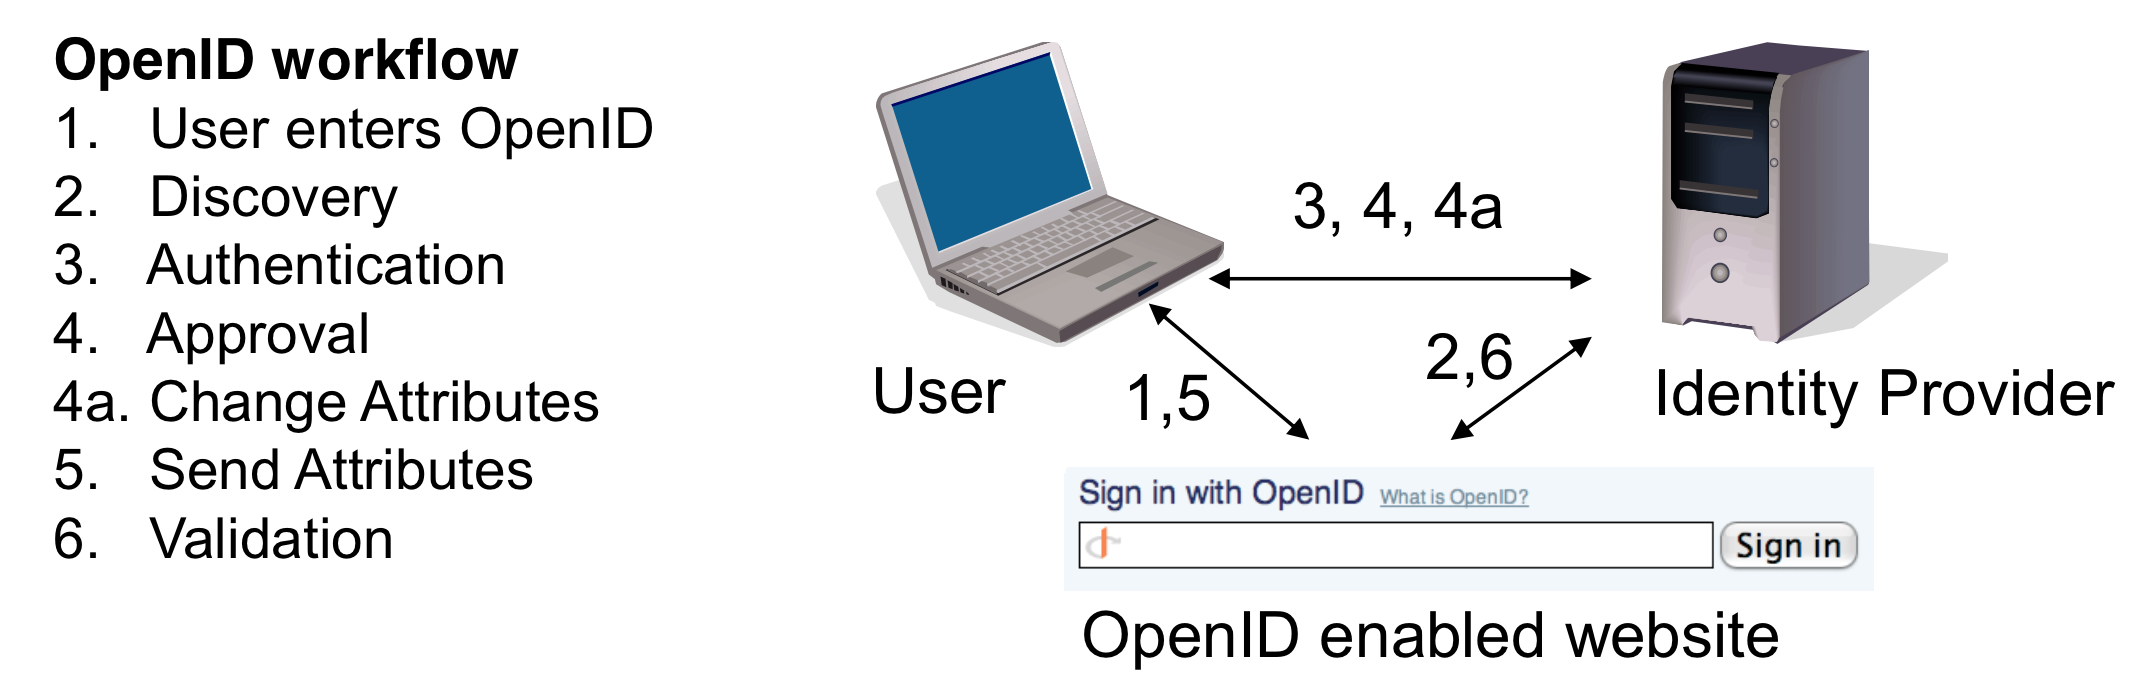
\includegraphics[width=\columnwidth]{img/OpenID.png}
  }
  \sectionbox{
  \subsubsection{OAuth}
    A web user (resource owner) grants a
    printing service (client) access to her protected photos stored at a photo sharing service (resource server), without sharing her username and password with the printing service.
    Instead, she authenticates directly with a server trusted by the photo sharing service (authorization server) which issues the printing service delegation-specific credentials (access token).

    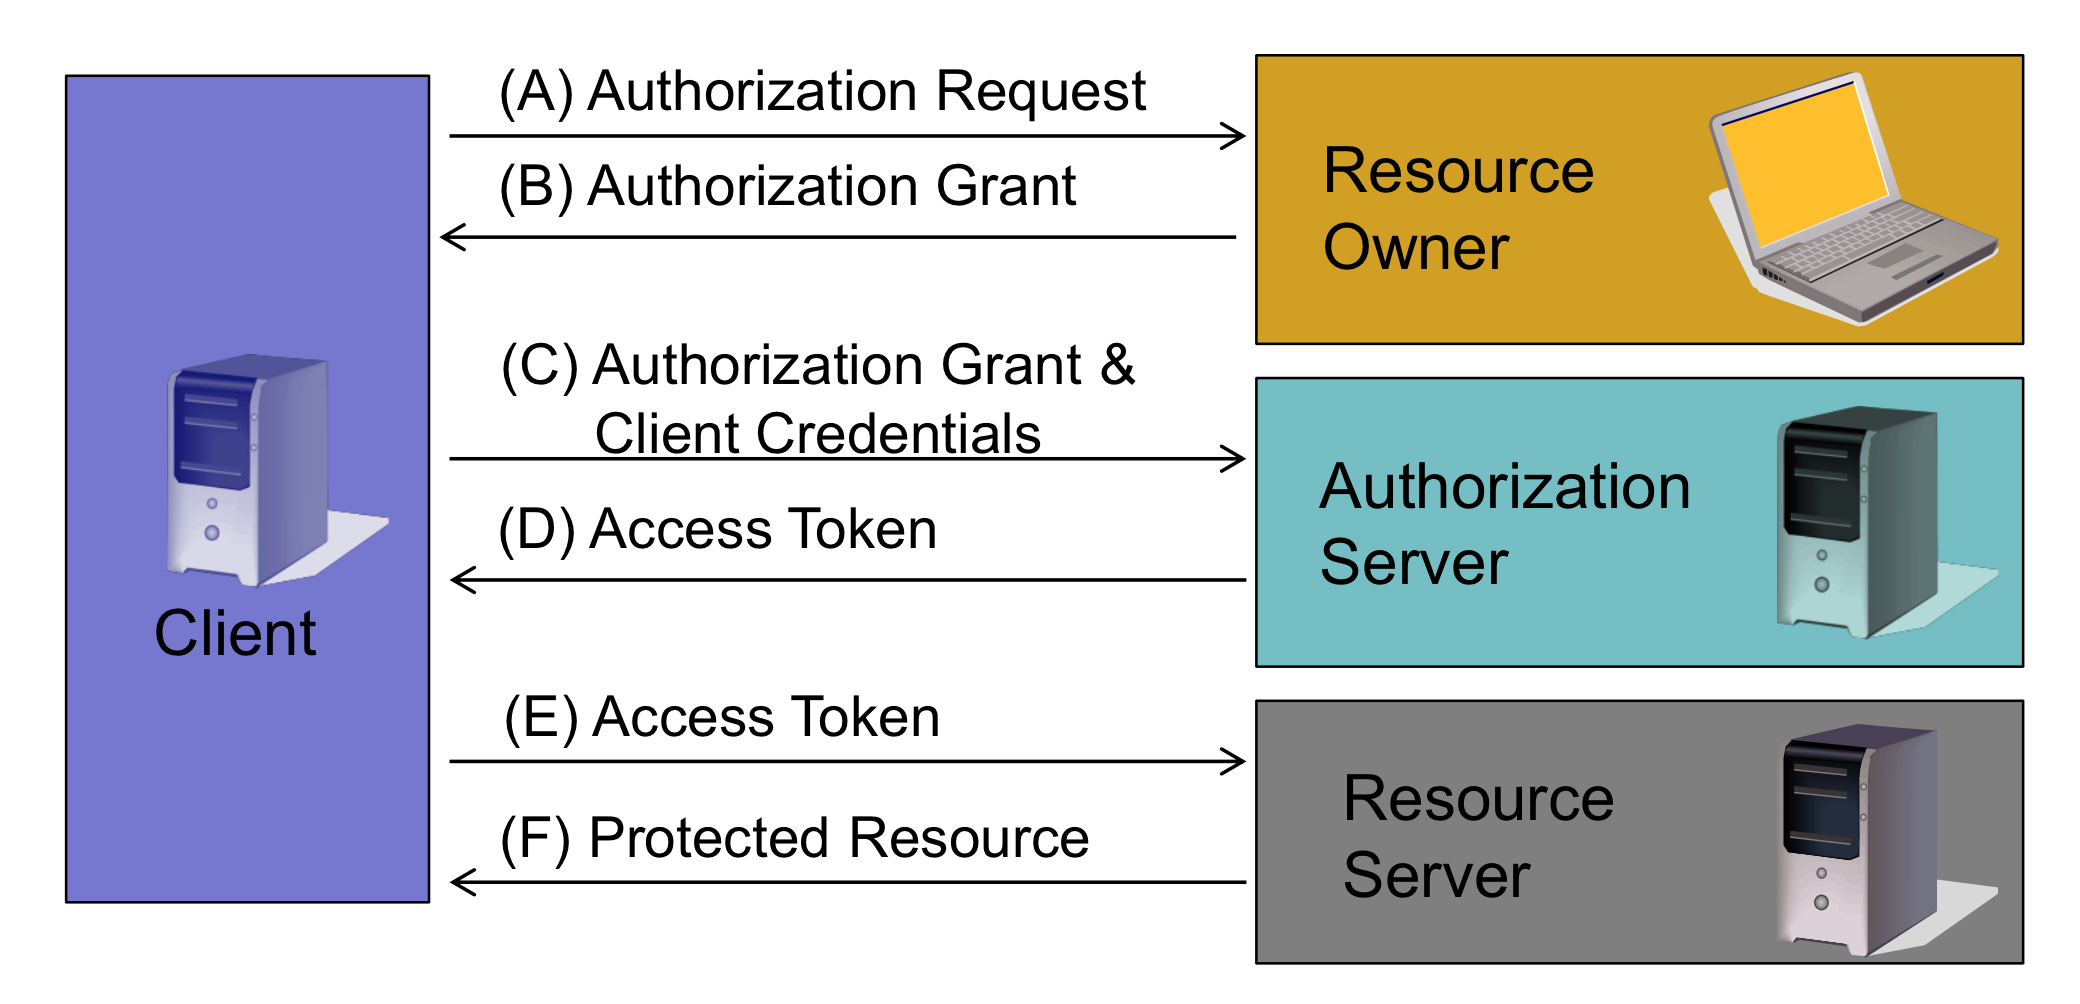
\includegraphics[width=\columnwidth]{img/OAuth.png}

    (A) Client requests authorisation from the resource owner or authorization server. \\
    (B) Client receives an authorisation grant by the resource owner. Authorization grant type depends on the method used by the client and supported by the authorisation server to obtain it. \\
    (C) Client requests an access token by authenticating with the authorization server using its client credentials (prearranged between the client and authorization server) and presenting the authorization grant. \\
    (D) Authorisation server validates  client credentials and the authorisation grant, and if valid issues an access token.\\
    (E) Client requests protected resource from the resource server. Authentication by access token.\\
    (F) Resource server validates the access token \ra valid \ra serves request\\
  }
  \sectionbox{
  \subsubsection{3D Secure}
    A protocol used widely to authenticate online card transactions.

    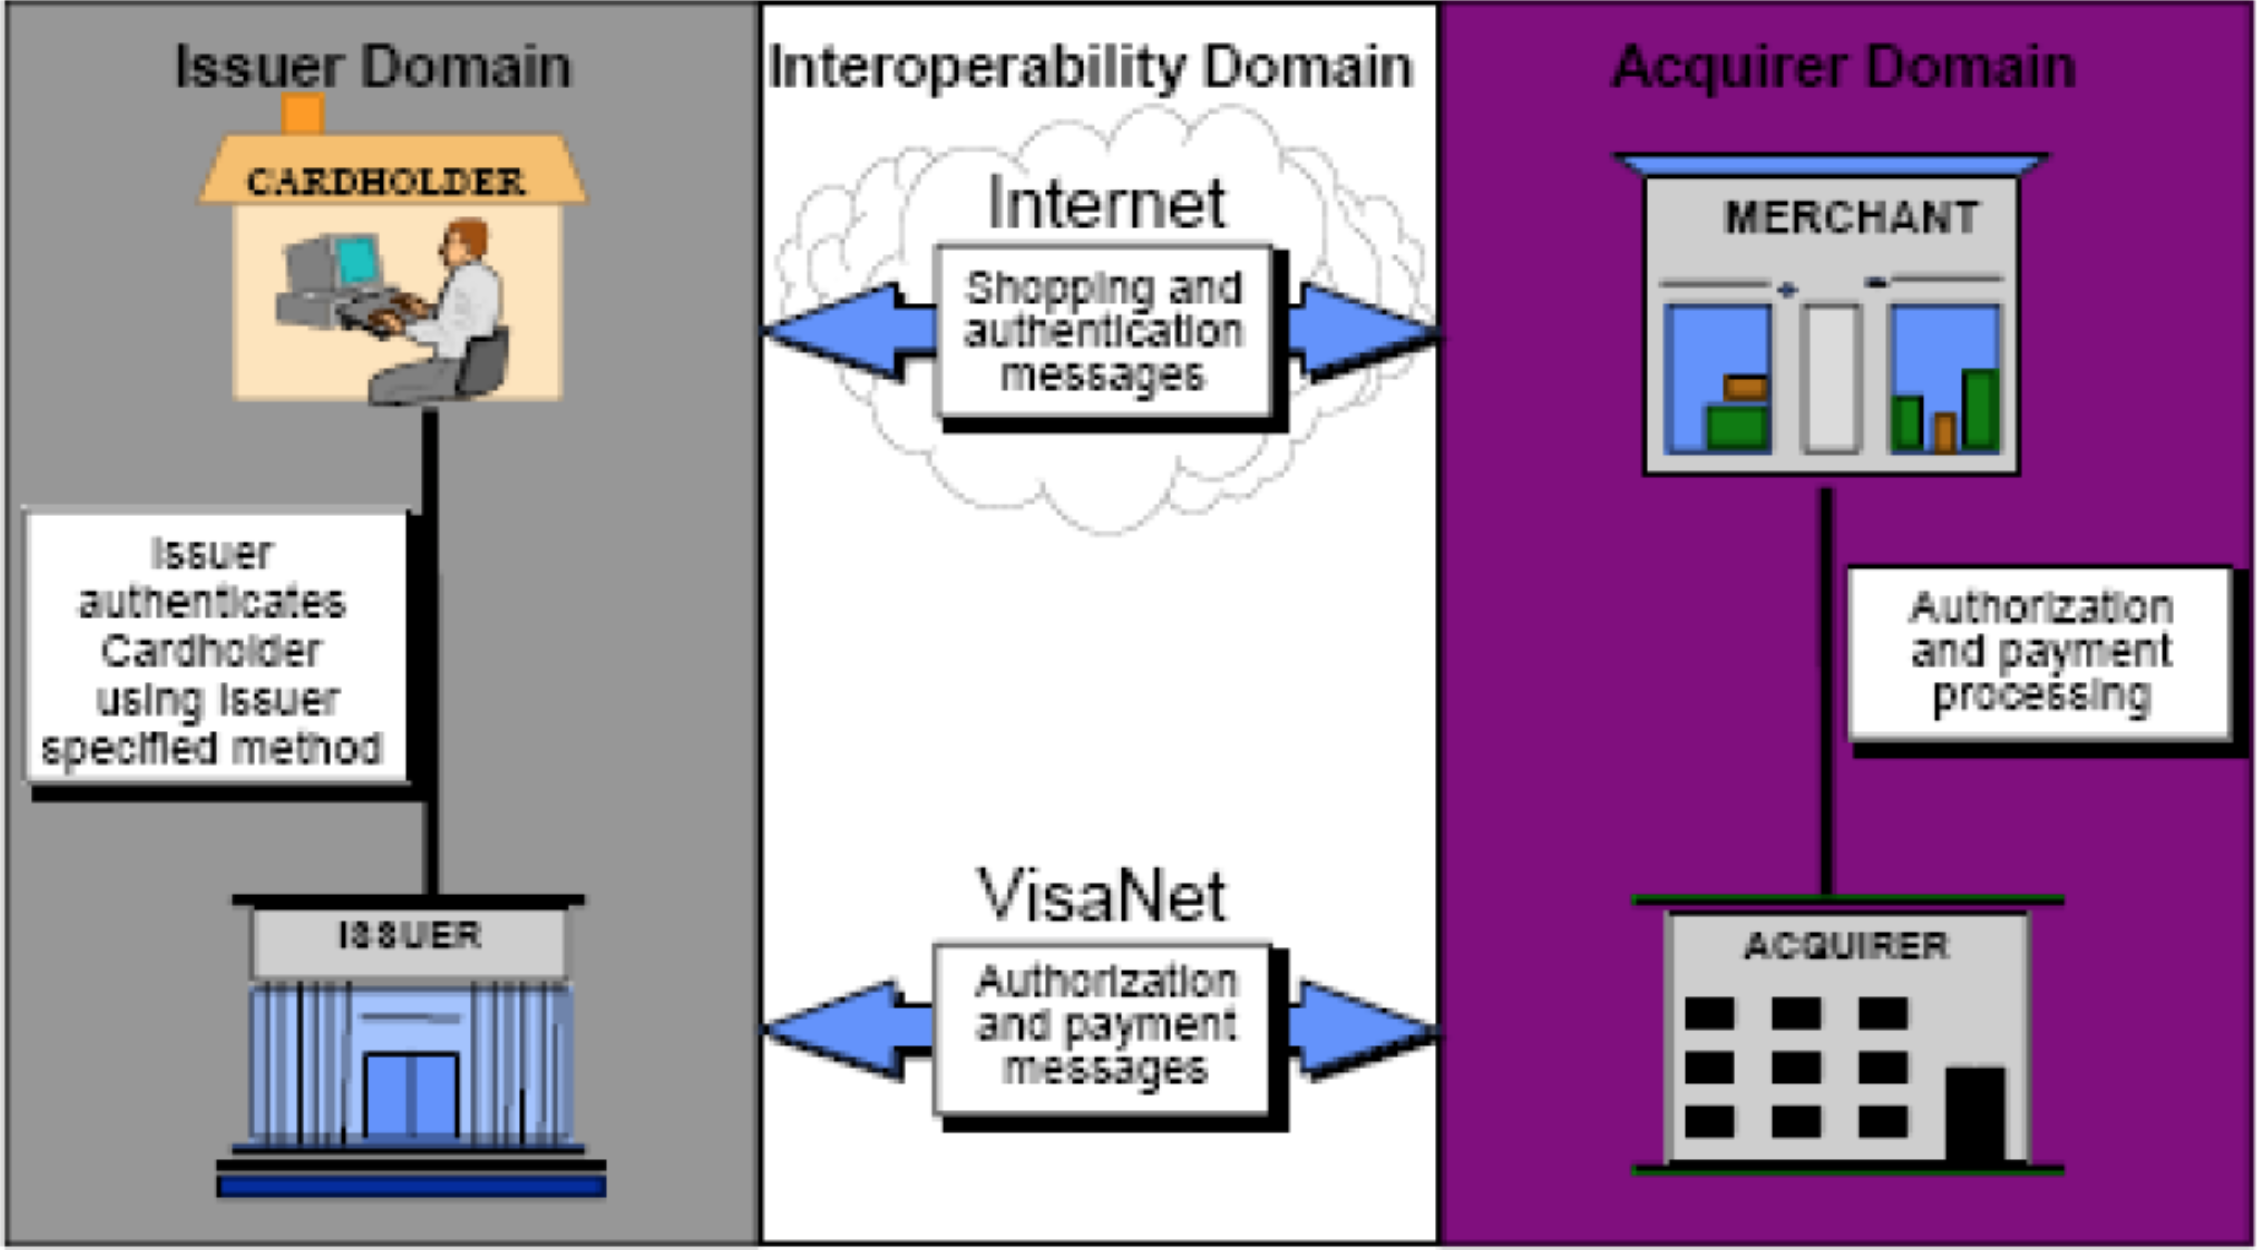
\includegraphics[width=\columnwidth]{img/3DSecure.png}
    After entering payment card details on merchant site:
    \begin{itemize}
    \item 3D Secure pops up a password entry form to a bank customer
    \item customer enters a password and, if it was correct,
    \item customer is returned to the merchant website to complete the
    transaction and
    \item the merchant gets an authorisation code to submit to his bank
    \end{itemize}

    \textbf{Problems:} Pop-Up blockers, Activation during shopping, SLL verification not visible, liability shift, weak bank authentication, no password reset procedure, privacy issues\\
  }
  \sectionbox{
  \subsubsection{802.1x}
    Client-server based access control protocol that restricts unauthorised devices from connecting to a (W)LAN through publicly accessible ports

    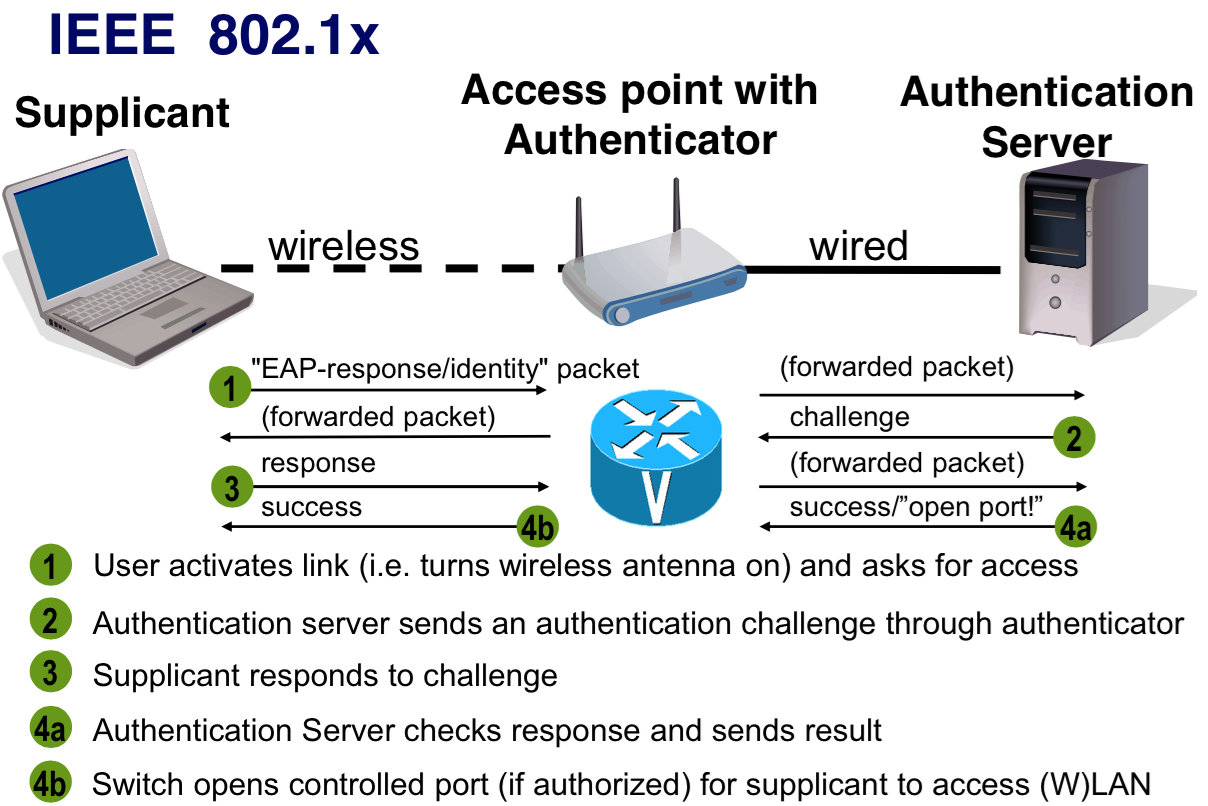
\includegraphics[width=\columnwidth]{img/8021x.png}

    \textbf{EAP} (Extensible Authentication Protocol): Authentication framework on the data link layer supporting multiple methods (MD5, OTP, TLS, TTLS) without requiring an IP.

    \textbf{Identity and Security}: Authentication (Who?) , Authorisation (What?) , Access Control, Policy enforcement

    \textbf{Benefits:} Standard based technology, control at link layer, interoperating wifi and wired, centralised user administration

    \textbf{Drawbacks:} Authenticator authentication, Man-in-the-middle, session hijacking
  }

  \sectionbox{
  \subsection{Anonymization}
    \textbf{Levels of Anonymity:} Identity (principal known), Pseudonymity (indirectly kown as pseudonym), anonymity (part of anonymity set but within no distinguishing)

    \textbf{Pseudonyms:} public (\ra identification), non-public (\ra pseudonymity), unlinkable (\ra anonymity)

    \textbf{Use cases:} \\
    physical: feedback, voting, whistleblowing, censorship \\
    digital: digital cash, digital voting, illegal activities

    \textbf{Oninon routing: } Data is encapsulated multiple times and only the next hop is known to each node

    \textbf{Mixnet:} proxy handles messages in batches (transformed and premutated) \Ra unlinkablity of incoming and outgoing messages

    \textbf{Attacks:} Traceback (break systems on path), Collusion (bad nodes), Traffic analysis (tagging with bit errors, replay messages - defense: heartbeats, traffic shaping, padding) , Logging (???)
  }


\section{Firewalls, IDS and NAT Traversal}
  \sectionbox{
  \subsection{Firewalls}
    Hardware or software device which is configured to permit, deny or proxy data through a computer network with different levels of trust. The configuration is called \emph{policy}.

    \textbf{Types:} simple packet filter, stateful filter, application layer proxy

    \textbf{Rules:} Filtering (outgoing (egress), incoming), Default (accept, reject), Deny (Drop, Reject), Addressing Transparency (firewall and network fingerprinting)
    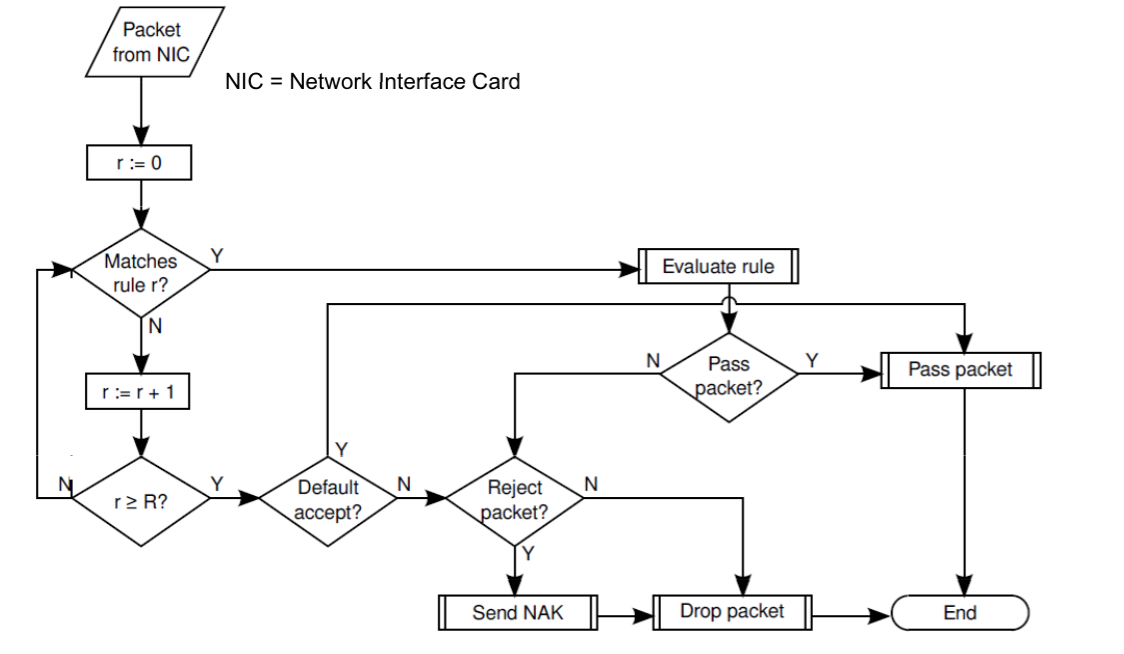
\includegraphics[width=\columnwidth]{img/firewallrule.png}

    \subsubsection{Stateless Firewall}
    Functionality: examine on network layer, decision based on header

    Pro: application independent, good performance

    Cons: no state or application context

    \subsubsection{Stateful Firewall}
    keeps track of state. Decision based on \emph{session state}

    Pro: more powerful

    Cons: no state for UDP, host vs. firewall state, state explosion

    \subsubsection{Application Layer Firewall}
    take application state into account

    Pro: application aware

    Cons: many application protocols, performance

    \subsubsection{Web Application Firewall}
    protects web-based applications from malicious requests (often reverse proxy)

    Filtering: signatures, black/whitelisting
    } \sectionbox {
    \subsection{Firewall Attack techniques}
    \begin{itemize}
    \item IP source spoofing
    \item artificial fragmentation
    \item vulnerabilities
    \item Denial of Service (state explosion)
    \item Tunnelling/Covert channel (ICMP, DNS, \ldots)
    \end{itemize}
  } \sectionbox {
  \subsection{Firewall detection}
    Port scanning: traceroute, src IP of response

    TTL:  let expire TTL one hop past firewall
    } \sectionbox {
    \subsection{Oranizational challenges}
    \begin{itemize}
      \item Large rulesets
      \item Big Organisations
      \item Conflict: Networking vs. security staff
    \end{itemize}
  } \sectionbox {
  \subsection{IP Tables}
    Netfilter rule:
    iptables -A INPUT -i eth0 -m state --state ESTABLISHED, RELATED -j ACCEPT

    Iptables rule:  iptables -A INPUT -p tcp -s 0/0 -d 0/0 --destination-port 80 --syn -j ACCEPT
    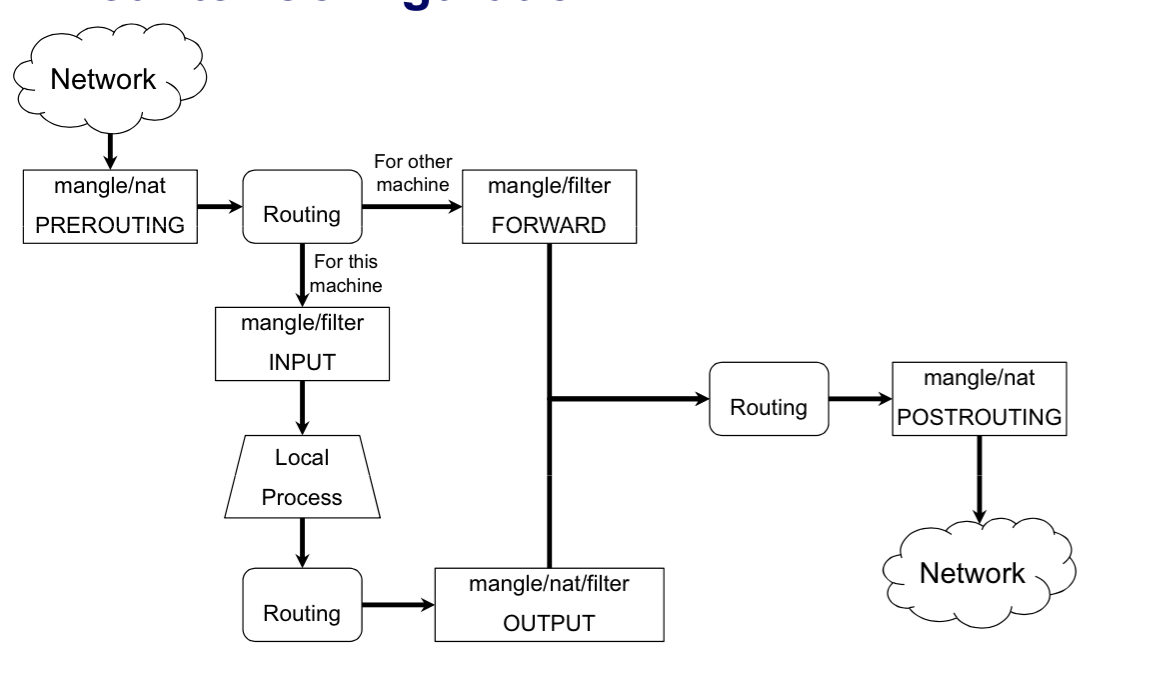
\includegraphics[width=\columnwidth]{img/netfilter.png}
   }
   \sectionbox {
   \subsection{NAT (Network Address Translation)}
    One way to the Internet (multiple hosts on private network using the same public IP address). IP Address rewriting.

    Benefits: Prevents malicous activity from outside, saves address space

    Drawbacks: no end-to-end connectivity, some protocols don't work

    \subsubsection{NAT UDP Hole Punching}

    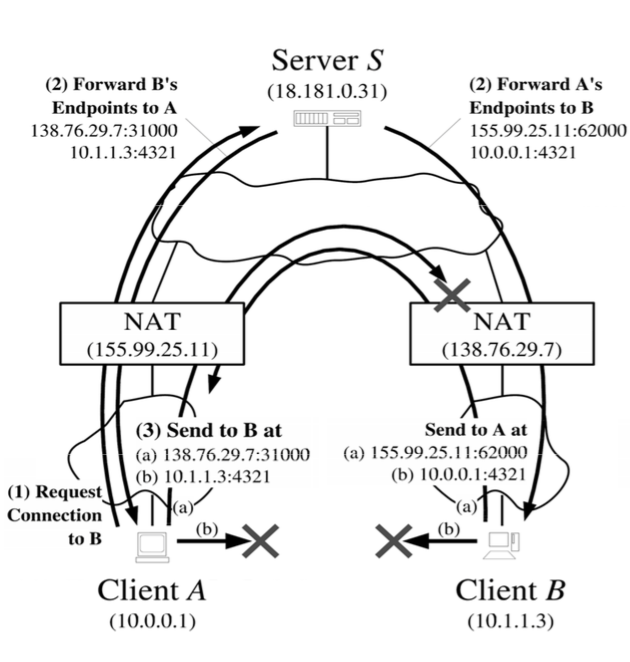
\includegraphics[width=\columnwidth]{img/nathole.png}
  }
  \sectionbox{
  \subsection{Intrustion Detection and Prevention Systems}
    try to detect intrusions on the network by comparing to attack signatures. Block traffic after detection.

    \subsubsection{Classification}
    \textbf{Object of observation:}

    Packet:

    Flow: scalabilty (+), encryption (+), not content-based (-)

    \textbf{Point of observation:}

    Host: hard deployment (-), context information (+), one sensore per machine (+)

    Network: easy deployment (+), multiple machines (+), unknown machines(-), preformance (-)

    \textbf{Method of observation:}

    Signature: precision (+), not detecting unknown attacks (-)

    Behavior: unknown attacks (+), difficult to find ground truth (-), false positives (-)

    \subsubsection{Challenges}
    \begin{itemize}
    \item false alarms
    \item high network speeds
    \item sensor management and signature distribution
    \item policy management
    \item manpower
    \end{itemize}

    \subsubsection{Attacks}
    \begin{itemize}
    \item Flooding / resource exhaustion
    \item algorithmic Complexity Attacks (e.g. on hash table)

    \end{itemize}
  }


\section{The Domain Name System Security}
  \sectionbox{
  \subsection{DNS}
    \emphbox{DNS is a global, distributed, robust system for name to IP address resolution}

    DNS is the glue of the internet: Nearly all activities start with a DNS lookup

    Orgiginally: no security considerations

    Design:
    \begin{itemize}
    \item Client-Server application
    \item Hierarchical System
    \end{itemize}

    \textbf{Zone:} Collection of hostnames/IP pairs managed together

    \textbf{Nameserver (authoritative): } Server that answers DNS queries (Responsible DNS Server for each zone)

    \textbf{Resolver:} Client part of DNS that resolves domain names

    \textbf{Recursive name server:}  Answers queries for all zones

    \textbf{Stub resolver:} Forwards request to recursive name server (typically used by end-hosts)

    \textbf{Caching:} Reduces overhead. Lifetime controlled by TTL
  }
  \sectionbox{
  \subsection{Attacks on DNS}
    \subsubsection{Denial of Service on DNS}
    Tageting the 13 DNS root servers which are a bottleneck resource. However overprovisioning (13 clusters) prevents most attacks.

    \subsubsection{Account-Takeover}
    Attacking the web interfaces of registrars and try to enter malicious name servers.

    \subsubsection{Manipulate local DNS settings}
    \begin{itemize}
    \item Manipulate local host configurations (access to the local machine nescessary)
    \item Spoof DHCP replies (access to LAN nescessary) \ra countermeasure: authentification for DHCP messages
    \item Set up Malicious DHCP server that is faster than the vaild one
    \end{itemize}

    \subsubsection{Manipulate DNS lookup process}

    \textbf{Bailiwick Checking:} Is the server authorized to respond to DNS requests for the domain.

    \textbf{Weak authentication:} Port, TXID, Query string - first good answer wins

    3 possible answers to DNS queries:
    \begin{itemize}
      \item Here is your answer
      \item go away
      \item I don't know ask \ldots
    \end{itemize}


    \subsubsection{The Kaminsky Attack}
    \begin{itemize}
    \item Inject query on the client Random.www.bank.com
    \item reply multiple times  (TXID 0-200)
    \item Send name server redirections
    \end{itemize}
    $\Ra$ Fix: Source Port Randomization. Chance: $65536 \cdot (65536 - 1024)$ to 1
  }

  \sectionbox{
  \subsection{DNSSEC}
    Provides:
    \begin{itemize}
      \item Authenticity
      \item Integrity
      \item Backward compatibility
    \end{itemize}

    Drawbacks
    \begin{itemize}
      \item No confidentiality
      \item No protection against DoS
    \end{itemize}

    All records are signed: Key pairs for each zone $\ra$ Integrity

    Chain of trust $\ra$ Authenticity
  }

\section{Availability and Denial of Service}
  \sectionbox{
  \subsection{System Level Agreements (SLA)}
    \begin{tabular}{ l | l | l }
      Level & Percentage & Downtime \\ \hline
      Two-nines & 99 & 3.5 days \\
      Three-nines & 99.9 & 9 hours \\
      Four-nines & 99.99 & 53 minutes \\
      Five-nines & 99.999 & 5 minutes \\
      Six-nines & 99.9999 & 31 seconds \\
    \end{tabular}

    How to achieve 99.999:
    \begin{itemize}
      \item High Redundancy
      \item Failure Resilience
      \item Over Provisioning
      \item Backup and Fast Recovery
    \end{itemize}
  }
  \sectionbox{
    \subsection{Denial of service}
    DoS: Resource starvation of CPU, Storage, Network

    Attacks:
    \begin{itemize}
      \item SYN-Flood: Spam Server with TCP SYNs $\rightarrow$ needs to keep state $\rightarrow$ Solution: Choose carefully constructed initial sequence number (crypto based)
      \item Compression Bomb
      \item Source Spoofing/Reflector Attack
      \item Mail Bounce: reply-to: @victim.com, To: and multiple Bcc: @target.com
      \item DNS Amplification: Send small request to recursive servers with spoofed source
    \end{itemize}
  }
  \sectionbox{
  \subsection{Dos Countermeasures}
    Prevention
    \begin{itemize}
      \item secure systems (e.g. prevent machine compromise to build bot
      nets by patching, IDS/IPS, firewall etc.)
      \item secure protocols (e.g. prevent IP spoofing, use TCP SYN
      cookies, HashCash: add client CPU cycles)
      \item resource accounting (server commits resources only to
      authenticated/trustworthy clients)
      \item resource multiplication (resource over provisioning for the case
      of an attack)
      \item late resource binding (bind resources as late as possible)
    \end{itemize}

    Reaction:
    \begin{itemize}
      \item detect (using pattern, anomaly, third party)
      \item react (rate-limit, filter, reconfigure, identify agents)
    \end{itemize}
  }

\section{Secure Channels: Principles, VPN, SSH}

  \sectionbox{
  \subsection{Security by Layer of the TCP/IP Model}
  Properties of a secure channel: secure = authentic and confidential

  \subsubsection{Security at Link Layer}
  \begin{itemize}
  \item All traffic over a specific Link
  \item Often implemented in hardware
  \end{itemize}

  Pro: Speed, Seamless

  Drawbacks: every link seperately, trust in link operator

  \subsubsection{Security at Internet Layer}
  secure traffic over multiple links between end points (e.g. IPSec)

  Pro: seamless security to above layers, IPSec part of IPv6 + IPv4

  Cons: complex configuration, tunnel mode encrypts only part of a route


  \subsubsection{Security at Transport Layer}
  e.g. TLS/SSL, SSH

  implemented in end-hosts

  Pro: can be added to existing apps, portable and easy configuration

  Cons (of TLS): protocol specific, application must be TLS/SSL aware


  \subsubsection{Security at Application Layer}

  implemented in end hosts (PGP, S/MIME, Skype, \ldots)

  Pros: extend app without involving OS, applications understand data

  Cons: seperate security for each app
  }

  \sectionbox{
  \subsection{VPN}
  connect networks or machines over an existing network

  \subsubsection{Tunnel mode}
  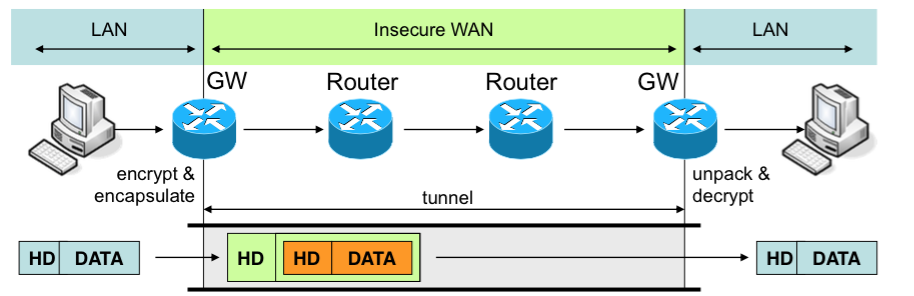
\includegraphics[width=\columnwidth]{img/vpntunnel.png}
  \begin{itemize}
  \item encrypt and authenticate orgininal IP packet
  \item transport htis as payload in new IP packet
  \end{itemize}
  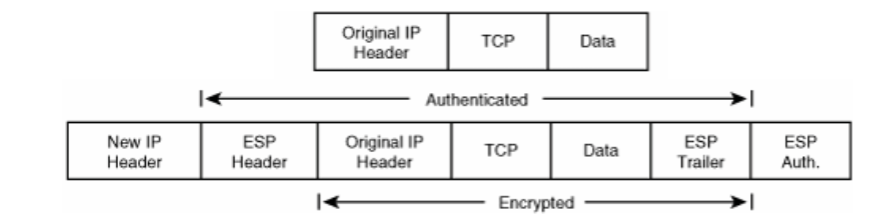
\includegraphics[width=\columnwidth]{img/vpntunnel2.png}
  \subsubsection{Transport mode}
  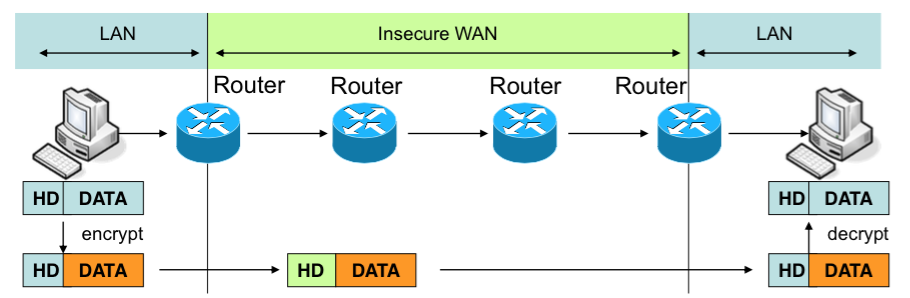
\includegraphics[width=\columnwidth]{img/vpntransport.png}
  \begin{itemize}
  \item end-to-end communication between hosts
  \item encrypt and authenticate payload only
  \end{itemize}
  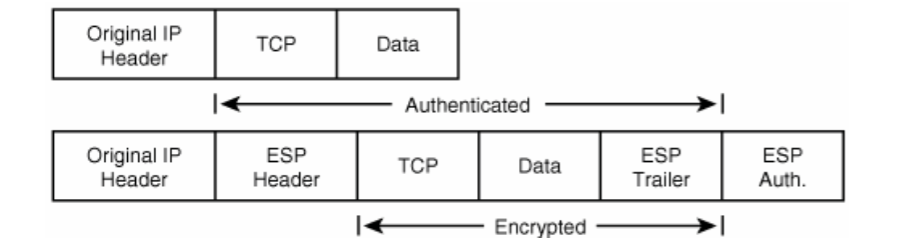
\includegraphics[width=\columnwidth]{img/vpntransport2.png}

  \begin{itemize}
  \item encryption
  \item randomized IVs
  \item replay protection
  \item authentication (HMAC)
  \end{itemize}

  \subsubsection{Security Association (SA)}
  A Security Association (SA) is the establishment of shared security attributes between two network entities to support secure communication. An SA may include attributes such as: cryptographic algorithm and mode; traffic encryption key; and parameters for the network data to be passed over the connection.
  } \sectionbox{
  \subsection{Message Authentication Code (MAC)}
  Provide data and integrity
  \begin{itemize}
  \item message not modigied in transit
  \item source is authentic
  \item not delayed
  \item sequence order
  \end{itemize}

  MAC (K, M) = DES (K, M) take last 32 bits

  \subsubsection*{HMAC (Mac with Hash functions)}
  \begin{itemize}
  \item use hash functions (MD5, SHA)
  \item faster
  \item easy availible
  \end{itemize}

  HMAC (K, M) = H(K' xor opad | H (K' xor ipad | M))


  } \sectionbox{
  \subsection{SSH}
  standard for remote login and encrypted file transfer

  \subsubsection{Protocols}
  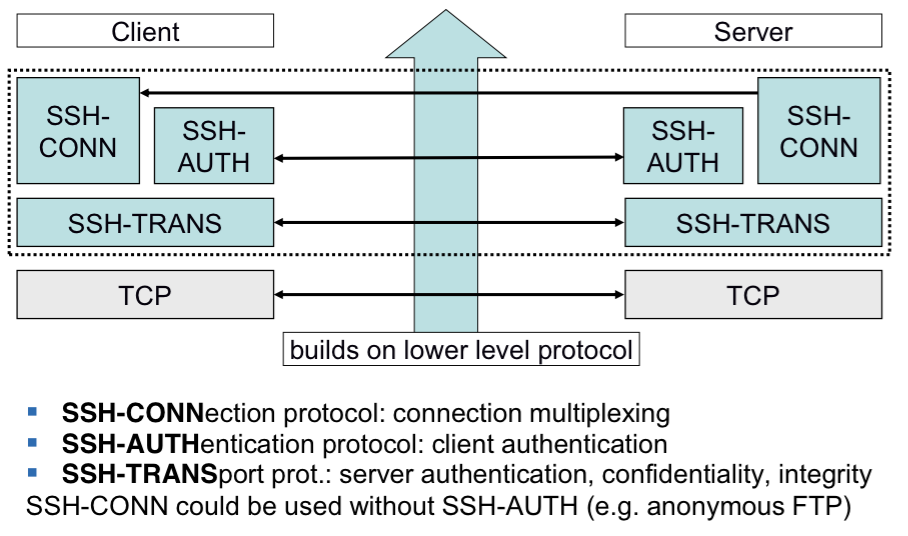
\includegraphics[width=\columnwidth]{img/sshproto.png}

  \subsubsection{SSH-Trans}
  \begin{itemize}
  \item algorithm negotiation
  \item session key exchange (e.g. Diffie-Hellman)
  \item session id
  \item server authentication
  \item encryption, integrity, data compression
  \end{itemize}

  \subsubsection{SSH-Auth}
  \begin{itemize}
  \item authenticates the client with multiple auth mechanisms
  \item defines format of auth-requests (Username, Method name, Service name)
  \end{itemize}

  \subsubsection{SSH-Conn}
  \begin{itemize}
  \item multiplexing multiple steams
  \item port forwarding
  \item compression handling
  \item interactive and non-interactive sessions
  \end{itemize}


  \subsubsection{Attacks}
  \begin{itemize}
  \item password cracking
  \item traffic analyis
  \end{itemize}
  }
  % Network layers (and security in different layers)
  % VPN technologies (building blocks, IPSec)
  % SSH (algorithms parameters)
  % Passwords

\section{TLS}
  Cipher Suite = key exchange + cipher spec

  \sectionbox{
  \subsection{Key Exchange Methods}
  \begin{itemize}
  \item RSA:  secure against PA, AA, no PFS, no cont. key agreement
  \item RSA with temp. pub/priv: secure against PA, AA, PFS, no cont. key agreement
  \item Fixed DH: secure against PA, AA, no PFS, cont. key agreement
  \item Ephemeral DH: secure against PA, AA, PFS, cont. key agreement
  \item Anonymous DH: secure against PA, not against AA, PFS, cont. key
  \end{itemize}
  } \sectionbox{
  \subsection{DH key agreement}
  \begin{itemize}

    \item Public	values:	large	prime	p,	generator	g
    \item Alice	has	secret	value	a,	Bob	has	secret	b
    \item A	$\rightarrow$ B:	$g^a$	(mod	p)
    \item B	$\rightarrow$ A:	$g^b$  (mod	p)
    \item Bob computes	$(g^a)^b$	=	$g^{ab}$	(mod	p)
    \item Alice	computes $(g^b)^a$	=	$g^{ab}$	(mod	p)
  \item Eve	cannot	compute	$g^{ab}$	(mod	p)
  \end{itemize}
  } \sectionbox{
  \subsection{TLS session}
  Sample TLS Session (no client auth):
  \begin{itemize}
  \item C $\rightarrow$ S:  client\_hello
  \item S $\rightarrow$ C:  server\_hello: Ephemeral DH  key exchange,   RC4 encryption,  MD5-based   MAC
  \item S $\rightarrow$ C:  Server  certificate, containing  RSA public  key : Client checks  validity + verifies URL matches certificate!
  \item S $\rightarrow$ C:  Server\_key\_exchange: g, p, $g^s$, ${H(g, p, g^s)}_{KS^-1}$
  \item S $\rightarrow$ C:  server\_hello\_done
  \item C $\rightarrow$ S:  client\_key\_exchange: $g^c$
  \item C $\rightarrow$ S:  change\_cipher\_spec
  \item C $\rightarrow$ S:  finished
  \item S $\rightarrow$ C:  change\_cipher\_spec
  \item S $\rightarrow$ C:  finished
  \end{itemize}

  Phase 1: (Client,Server)\_hello\_message:
  \begin{itemize}
  \item Highest   supported   version
  \item Random    =   32  bit Timestamp  $||$  28  bytes   random
  \item Session   id
  \item Client\_hello: Supported   cipher  suite,  ciphers are listed
  in  decreasing  order   of  preference
  \item Server\_hello: chosen  cipher
  \end{itemize}

  Phase 2:  Server  authentication    and key exchange
  \begin{itemize}
  \item S $\rightarrow$ C:  certificate
  \item S $\rightarrow$ C:  server\_key\_exchange: Anonymous DH, Ephemeral   DH, RSA key exchange    with    sign-only   key
  \item S $\rightarrow$ C:  certificate\_request: Cert\_type (RSA    or  DSS for key exchange); List  of  acceptable  certificate  authorities
  \item S $\rightarrow$ C:  server\_hello\_done
  \end{itemize}

  Phase 3:  Client  authentication and key exchange
  \begin{itemize}
  \item C $\rightarrow$ S: client\_key\_exchange: RSA: client generates 48  byte pre-master  secret, encrypts it  with server’s
  public  key; Eph or  anon DH: client  public  DH  value; Fixed DH: null (certificate contained DH  key)
  \end{itemize}

  Phase 4: Finish
  \begin{itemize}
  \item C $\rightarrow$ S: change\_cipher\_spec: Establish set up cipher and keys
  \item C $\rightarrow$ S: finished: MD5( master\_secret $||$ pad2 $||$ MD5( handshake messages $||$ Sender $||$ master\_secret $||$ pad1 )) $||$ SHA-1( master\_secret $||$ pad2 $||$ SHA-1( handshake messages $||$ Sender $||$ master\_secret $||$ pad1 )); Handshake messages contains all messages up to now
  \item S $\rightarrow$ C: change\_cipher\_spec
  \item S $\rightarrow$ C: finished
  \end{itemize}
  }


\section{Web Application Security: Session State}
  \sectionbox {
  \subsection{Anatomy of Web App}
  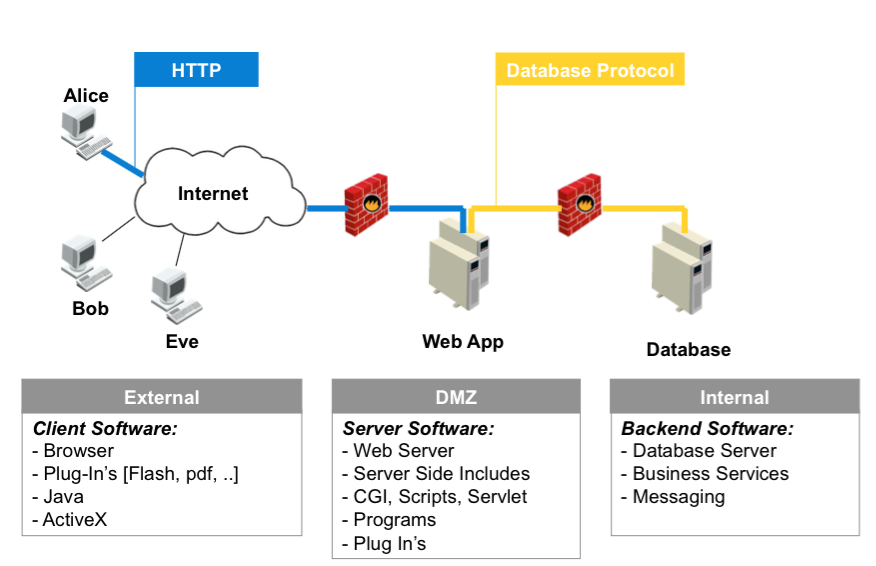
\includegraphics[width=\columnwidth]{img/webapp.png}
  } \sectionbox {
  \subsection{Threat vectors}
  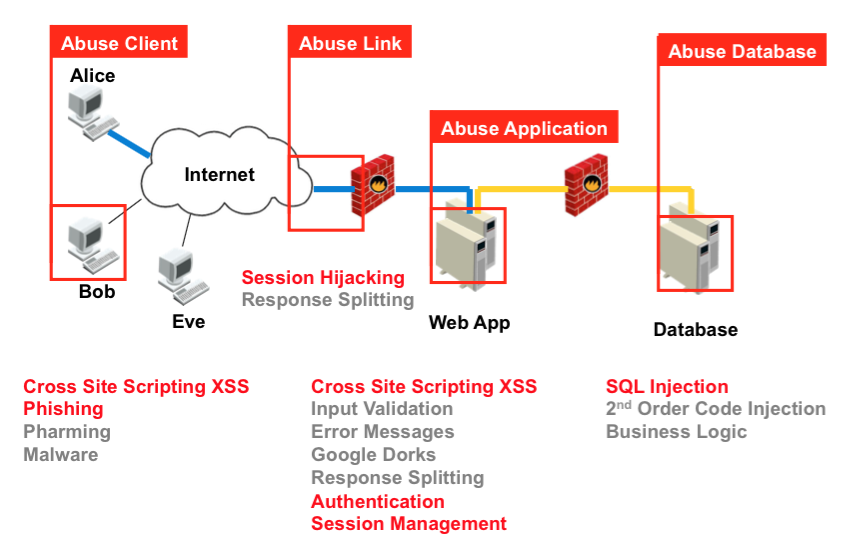
\includegraphics[width=\columnwidth]{img/threatvectors.png}

  } \sectionbox {
  \subsection{HTTP  and Session management}
  HTTP is stateless $\ra$ state needs to be implemented with session ID

  SessionID: needed for state, generated on the server, stored on the client, transmitted for every request

  Crucial processes: Generation, Transport, Destruction, Revocation

  \subsubsection{Possible transport ways}
  \begin{itemize}
  \item GET: easy, compatible (+) , logged, referer (-)
  \item POST: compatible, not obvious (+), more complex development, slightly harder to manipulate (-)
  \item Cookie: more option, not recorded, https restriction (+), internet cafes, may be disabled by users (-)
  \end{itemize}

  \subsubsection{Generation} strong random value

  \subsubsection{Revocation}
  Session validity: client and server side revocation, session information time limited

  Session timeout: extremely imported for shared computers, expiry time should be kept to minimum
  } \sectionbox {
  \subsection{Attacks}
  \begin{itemize}
  \item Network sniffing $\ra$ HTTPS
  \item Do not mix HTTP and HTTPS sessions
  \item Random SessionID is important
  \end{itemize}
  }

%Web Application Security: SQL Injection
\section{Web Application Security: SQL Injection}
  \sectionbox{
  \subsection{Code Injection}
  \textbf{Code injection:} Code injection refers to attacks which insert code that is afterwards interpreted by a process

  \textbf{Code injection process:}
  \begin{itemize}
  \item Data enters app from untrusted source
  \item Data is part of a string executed as a command by app
  \item app gives the attacker a privilege or capability that the attacker would otherwise not have
  \end{itemize}
  } \sectionbox{
  \subsection{SQL code injection}
  A SQL injection attack consits of insertion of a SQL query via the input data from the client to the application.

  Possible causes:
  \begin{itemize}
  \item read / modify data in the database
  \item execute administration opertations
  \item issue commands on the OS
  \end{itemize}

  \textbf{Example:} \lstinline|$login="' or ''=''"|

  \lstinline|;| terminates a command \lstinline|--| considers everything afterwards as a comment.

  \lstinline|union| merges the output of two select commands.

  Error messages can provide hints on which DB is used.

  \textbf{IDS Detection} can be avoided by varying the command (e.g. through the insertion of whitespaces)
  } \sectionbox{
  \subsection{SQL Injection Defense}
  \begin{itemize}
  \item constrain and sanitize all client data on the server
  \item use stored procedures
  \item avoid disclosing error information
  \item run DB with reduced privileges
  \item input validation
  \end{itemize}
  } \sectionbox{
  \section{Cross-Site Scripting (XSS)}
  \subsection{Same-origin policy}
  A script can only access content and properties of a document loaded from the same origin.
  \begin{itemize}
  \item same protocol
  \item same hostname
  \item same port
  \end{itemize}
  URL path is ignored for the same-origin policy

  \textbf{Interaction of different origins}
  \begin{itemize}
  \item Link
  \item Iframe: Shown inside me.tld but cannot exit iframe
  \item POST: POSTing data to you.tld
  \item script include: Evaluted in context of me.tld ($\ra$ dangerous)
  \item Asynchronous Requests (AJAX): Different origin only possible if allowed by target domain (with Access-Control-Allow-Origin Header)
  \end{itemize}
  } \sectionbox{
  \subsection{Cross-Site Scripting (XSS) Attacks}
  XSS flaws occur whenever a web app takes user supplied data and sends it to the browser without first \emph{validating} or \emph{encoding} the content.

  \textbf{Target:} The user of the app insted of the app itself

  \textbf{Infection path:} email, chat, uploaded files \ldots

  \textbf{Dangerous content:} advertisments, user contributed content, widgets (counters, scripts \ldots)
  } \sectionbox{
  \subsection{XSS prevention}
  \begin{itemize}
  \item test your web app
  \item input sanitization (check user submitted content)
  \item HTML output encoding
  \end{itemize}
  } \sectionbox{
  \subsection{Data Leakage Attack}
  Attacker includes script that reads session cookies and sends them to an evil server. $\ra$ Solution: HTTPOnly cookies
  } \sectionbox{
  \subsection{Request Forgery (XSRF)}
  A form form one domain posts a request to a different domain through an authenticated session.

  \begin{itemize}
  \item write-only attack
  \end{itemize}

  \textbf{Solution:} CSRF Token, ask for password, check HTTP referer, show captcha
  } \sectionbox{
  \subsection{Script inclusion (XSSI)}

  \emph{Never include a script you do not trust!}

  Data is retrieved from the web server with a request on the API endpoint. The browser automatically sends cookie and the JavaScript function in the evil website is called with the AJAX return data.

  \textbf{Countermeasures:} security tokens derived from the cookie and a server challenge, use only HTTP POST, check HTTP referer
  }



% Malware
\section{Malware}

  \sectionbox{
  \subsection{Definitions}
  \textbf{computer virus} is computer program which does: infection, propagation, mutation (polymorphism), executing malcode

  \textbf{Malicious software (Malware)} is software that is intentionally included or inserted in a computer system for a harmful purpose.

  \textbf{Trojan} seemingly offers usefu functionality but contains hidden functionality which undermine system security

  \textbf{Worm:} Software that can replicate itself from computer to computer across network connections

  \textbf{Bot:} malicious software agent running on a compromised machine executing commands by the bot master by listening to the command and control center

  } \sectionbox{
  \subsection{Malware on portable storage}

  \begin{itemize}
  \item uses sneakernet as non-local propagation
  \item variants: boot code virus (replaces boot sector), host program infection (embedding into executables)
  \end{itemize}
  } \sectionbox{
  \subsection{Problem of malware}

  \begin{itemize}
    \item Unauthorized use of system/network resources
    \item Sabotage
    \item Espionage
    \item Lowering of system security
  \end{itemize}
  } \sectionbox{

  \subsection{Malware detection}

  \textbf{Goal:} Detect malware and disinfect system

  \textbf{Deployment:} endpoint, network

  \textbf{Evaluation:} recognition rate (high true positive), false alarm rate


  \subsubsection{Signature Based}
  \begin{itemize}
    \item Reactive (based on known malware binaries)
    \item Signature database (keeps growing, polymorphism)
    \item Metrics: update delay, coverage, resource consumption
   \end{itemize}

     \subsubsection{Behaviour Based}
  \begin{itemize}
    \item requires bahaviour model (ground truth, baseline)
    \item problematic: user alerting
   \end{itemize}

   \subsubsection{Evaluating Antivirus products}

   \begin{itemize}
      \item Detection (reactive, proactive)
      \item support for compression
      \item self-protection
      \item cleanup
      \item enterprise deployment features
    \end{itemize}
  } \sectionbox{
    \subsection{Advanced Presistent Threat}
    Sophisitcated stealth customized attack on selected high value targets
    \begin{itemize}
      \item Advanced: sophisticated attack techniques
      \item Persistent: might launch any time and hide well, hard to detect
      \item Threat: specific objective, skilled, well funded
     \end{itemize}
  } \sectionbox{
     \subsection{Antivirus Detection Evasion}
     \begin{itemize}
        \item Polymorphism
        \item code obfuscation
        \item encryption of code
        \item code changes to prevent disassembly
        \item sandbox detection
        \item bootstrapping / multi stage
      \end{itemize}
  } \sectionbox{

      \subsection{Worm Propagation Mechanism}
      \begin{itemize}
        \item Select a target
        \item contact target
        \item check if target is vulnerable
        \item exploit
        \item install copy of worm
        \item start copy
       \end{itemize}

       Propagation speed: scan rate, vulnerable population, system compromise delay, worm transfer speed


       \subsubsection{SIS Model}
       SIS: susceptible infected susceptible
       \begin{itemize}
          \item two states: susceptible and infected
        \end{itemize}

        $\rho (t)$ fraction of infected nodes \\
        $\beta$: infection rate \\
        $\delta$: cure rate\\
        $k$: number of outgoing edges at each node\\
        $\diff \rho (t) / \diff t = \beta k (1 - \rho (t)) \rho (t)  - \delta \rho (t)$\\
  } \sectionbox{
        \subsection{Worm Network Impact}
        \begin{itemize}
          \item ARP flooding
          \item ICMP destination unreachable
          \item higher network and traffic flows
         \end{itemize}
  } \sectionbox{
         \subsection{Malware countermeasures}
         \begin{itemize}
            \item End system: patching, firewall, IPS, Antivirus
            \item Anti-Virus: useful but not too effective
            \item Monocultures are targeted first
            \item Slow patching is a huge risk
            \item Application whitelisting
            \item No trusted intranet
            \item Thin Client (e.g. ChromeOS)
          \end{itemize}

          }

% Botnets
\section{Botnets + Malware Development and Demo}
  \sectionbox{
  \subsection{Objectives}
  \begin{itemize}
    \item Buildup efficient infection and spreading
    \item prevent detection and removal
    \item address changing functionality needs
    \item handle large number of machines
    \item to business and technology challenges
    \item Anonymity prevent identification of operator
  \end{itemize}
  } \sectionbox{
  \subsection{Target exploitation}
  \begin{itemize}
  \item Persist and avoid detection (explore, steal information, load functionality, maximize yield)
  \item Move to active attacks (load attack functionality $\ra$ higher chance of detection)
  \item Throw away agent (sell to idiots)
  \end{itemize}

  } \sectionbox{
  \subsection{Bot command modes}

  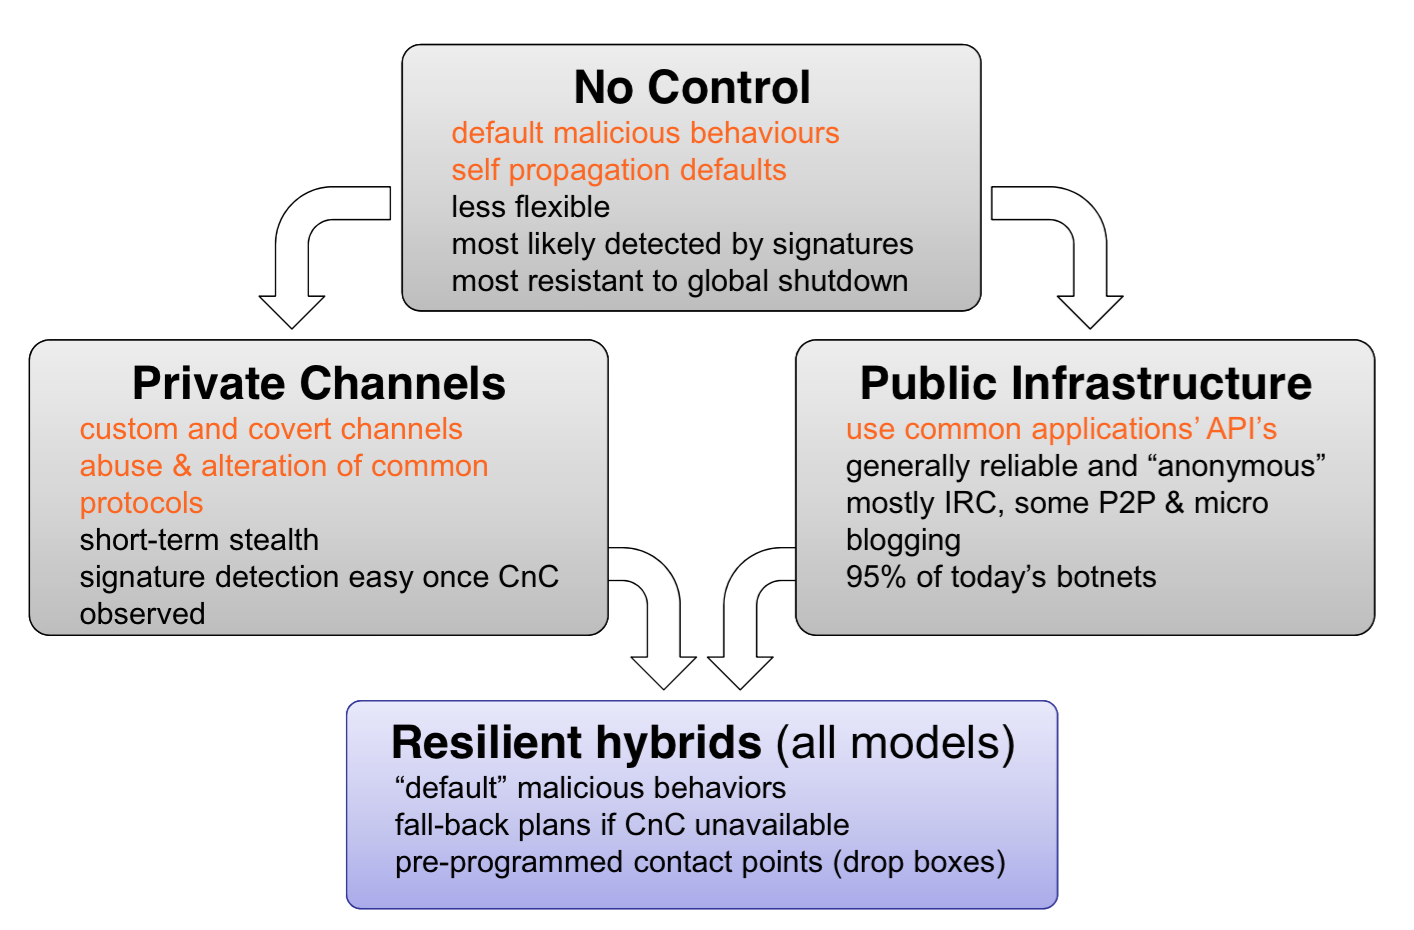
\includegraphics[width=\columnwidth]{img/bot-command-modes.png}
  } \sectionbox{
  \subsection{Exploitation Phases}
  \begin{itemize}
    \item ID Theft
    \item Peer and Social Attacks (Trust misuse)
    \item Local Attacks (Local Network, USB)
    \item Attack Support (Host of Phising Site)
    \item External/Noisy Attacks (Scanning, Spam, DDoS)
  \end{itemize}

  \textbf{CnC Topologies:} Star, multi-server, hierarchical, random
  }

  \sectionbox{
  \subsection{Fluxing Technologies}
  \begin{itemize}
    \item IP-Flux: Constant change of IP address information related to a particular fully-qualified domain name (FQDN)
    \item Domain Flux: Constant change and allocation of multiple fully-qualified domain names (FQDN)
    \item Single-Flux: The FQDN of the CnC’s host has multiple IP addresses assigned (DNS A record)
    \item Double-Flux: The name servers of the CnC’s FQDN as well as the FQDN of the CnC’s host have multiple IP addresses assigned (DNS A and NS records)
  \end{itemize}
  }

  \sectionbox{
  \subsection{Malware Development Process}
  Develop, Crypt, Protect, Pack, Bind, QA

  }

  \sectionbox{
  \subsection{Detection Evasion Tactics}
  \begin{itemize}
    \item Create unique samples of malware at massive scale
    \item Protect malware from analysis
    \item Detect sandboxing
    \item Test detectability before deployment
   \end{itemize}
  }

  \sectionbox{
  \subsection{Takedown}
  legal and technical measures to sever the connection  between the CnC stucture the bot agents
  }

  \sectionbox{
  \subsection{Defense}
  \begin{itemize}
    \item Firewalls
    \item Antivirus (up-to-date), know limits
    \item patch
    \item brain.exe
   \end{itemize}

  }


% Security Ecosystem and Detection Failures
\section{Security Ecosystem and Detection Failures}

  \emphbox{A vulnerability is a weakness in software (or hardware) that enables an attacker to compromise the software or the data that it processes}
  \sectionbox{
  \subsection{Security Information Provider}
    SIP: Organizations that efficiently monitor the primary sources of security information, validate the content found, and publish their findings as security advisories in a consistent format (NVD, CVE)
  }
  \sectionbox{
    \subsection{Disclosure Options}
    \begin{itemize}
      \item Exploit
      \item Sell on Black Market
      \item Full Disclosure
      \item Coordinated/Responsible Disclosure
      \item Sell on White Market
    \end{itemize}
  }

% E-Mail Spam
  \section{E-Mail Spam}
  \sectionbox{
  \subsection{Define Spam}
    \textbf{UCE}: Unsolicited Commercial Email

    \textbf{UBE}: Unsolicited Bulk Email (not nescessaryliy commercial)
  } \sectionbox{
  \subsection{Blacklists}
    How Realtime Blacklists Lists Differ:
    \begin{itemize}
      \item Nomination (how to get on the list)
      \item Listing lifetime (how to get off the list)
      \item Cost
      \item Operator
      \item Goal
    \end{itemize}

    Blacklist Caveats:
    \begin{itemize}
      \item Blacklist evasion (spammer use botnet machines, stolen email accounts)
      \item Denial of service (if you are on blacklists $\rightarrow$ sucks)
    \end{itemize}
  }
  \sectionbox{
  \subsection{Email Auth}
    \begin{itemize}
      \item DomainKeys Identified Mail (DKIM): Pub/Priv Key Signing; pubkey distributed via DNS
      \item Sender Policy Framework: Domain owners publish list of IPs that are authorized
      \item SenderID: Match PRA domain against source IP via DNS (PRA is often From: header)
    \end{itemize}

    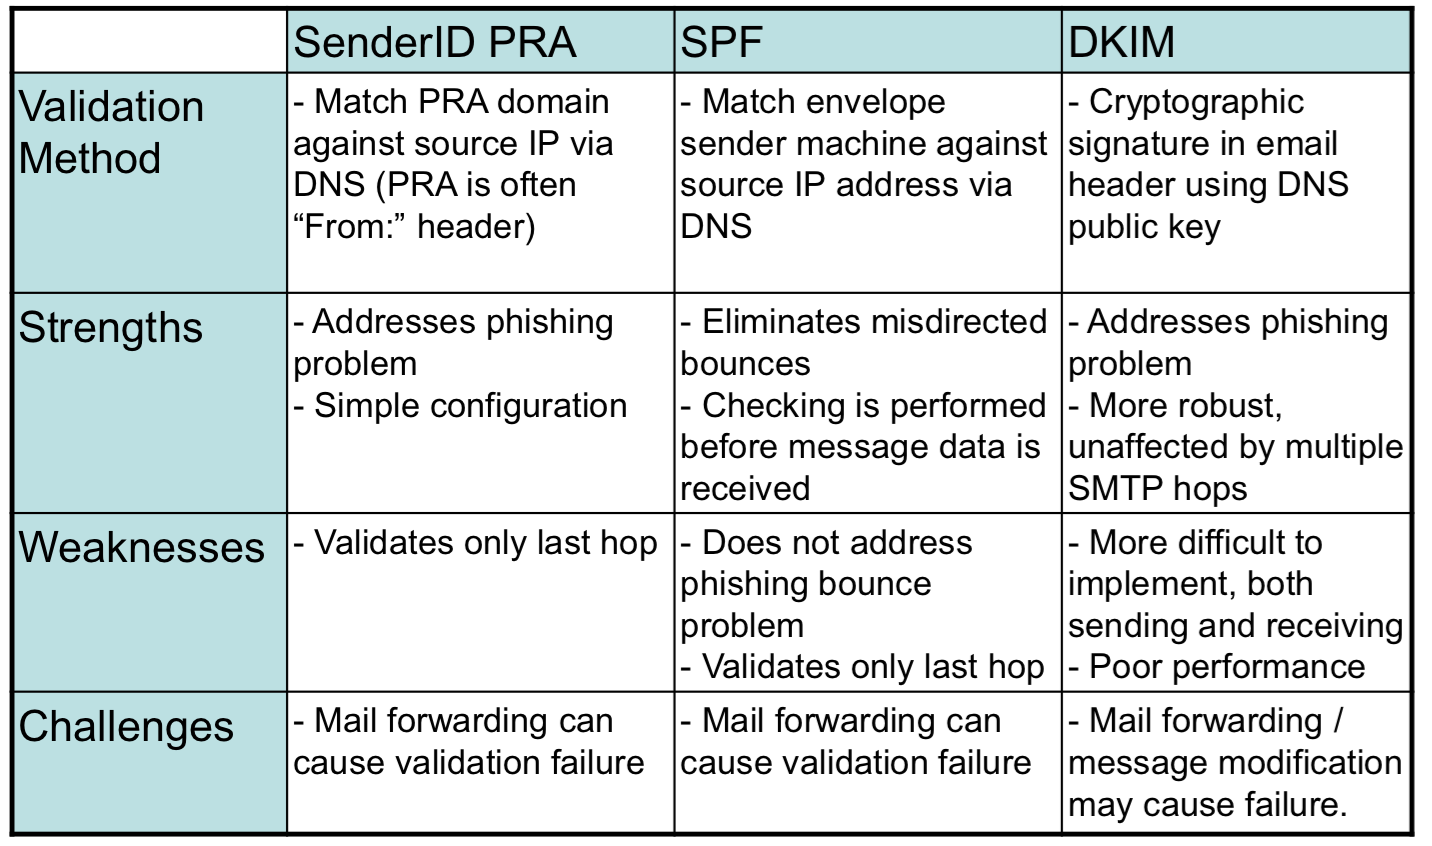
\includegraphics[width=\columnwidth]{img/emailauth.png}
  }
\section{Guest Lectures}
  \sectionbox {
  \subsection{DMZ}
    Compromised hosts in DMZ are no danger for internal network e.g.:(external - webserver(dmz) - database(internal))
  }
  \sectionbox {
  \subsection{Certificate Transparency  main goals}
    \begin{itemize}
      \item Make it impossible (or at least very difficult) for a CA to issue a SSL certificate for a domain without the certificate being visible to the owner of that domain.
      \item Provide an open auditing and monitoring system that lets any domain owner or CA determine whether certificates have been mistakenly or maliciously issued.
      \item Protect users from being duped by certificates that were mistakenly or maliciously issued.
    \end{itemize}
}

\end{document}
